\documentclass{article}
\usepackage[utf8]{inputenc}
\usepackage[a4paper, total={6in, 8in}]{geometry}
\usepackage{graphicx}
\usepackage{amsmath}
\usepackage{enumitem}

\title{Econ 20000-Problem Set 7}
\author{Dr. Fulya Ersoy}
\date{}
\begin{document}
\maketitle
\begin{enumerate}
\item (Based on Lima 11.4) Consider a consumer whose preferences for consumption (C) and leisure (R) are given by: $U(C,R) = \alpha lnC +(1-\alpha) lnR$. Suppose the consumer has T units of time that can be allocated to labor (L) and leisure (R). Let p denote the price of one unit of consumption and w denote the nominal wage
rate.
 \begin{enumerate}[label=(\alph*)]
\item  If M denotes consumer's non-labor income, write out the consumer’s budget constraint.
\item[] $L=T-R, \; pC=wL+M=w(T-R)+M\Rightarrow pC+wR=wT+M$.
\item Write out the Lagragian associated with this problem.
\item[] $\mathcal{L}=\alpha lnC+(1-\alpha)lnR+\lambda(w(T-R)+M-pC)$.
\item Derive the consumer’s labor supply function.
\item[] FOC's: $\begin{cases}
    \frac{\partial\mathcal{L}}{\partial C}=\frac{\alpha}{C}-\lambda p\Rightarrow\lambda=\frac{\alpha}{Cp}\\ \frac{\partial\mathcal{L}}{\partial R}=\frac{1-\alpha}{R}-\lambda w\Rightarrow\lambda=\frac{1-\alpha}{Rw}
\end{cases}$. $\Rightarrow \frac{\alpha}{Cp}=\frac{1-\alpha}{Rw}\Rightarrow\frac{C}{R}=\frac{\alpha }{(1-\alpha)}\cdot\frac{w}{p}$.
\item[] Let $k=\frac{\alpha }{(1-\alpha)}\cdot\frac{w}{p}$. Then $C=kR$. 
\item[] Using budget constraint: $p(kR)=w(T-R)+M\Rightarrow R(pk+w)=wT+M$.
\item[] $\Rightarrow pk=p\cdot\frac{\alpha }{(1-\alpha)}\cdot\frac{w}{p}=\frac{\alpha w}{1-\alpha}$. Thus $pk+w=w(\frac{\alpha}{1-\alpha}+1)=\frac{w}{1-\alpha}$. So $R=\frac{(1-\alpha)(wT+M)}{w}$.
\item[] Therefore $L^*=T-\frac{(1-\alpha)(wT+M)}{w}=\alpha T-\frac{(1-\alpha)M}{w}$ (Interior). Corner: $L^*=0$ if $L^*<0$.
\item For what value of M will the consumer supply positive hours of labor? How does consumer's labor supply decision vary with non-labor income, M?
\item[] Set $L^*>0$: $\alpha T-\frac{(1-\alpha)M}{w}>0\Rightarrow M<\frac{\alpha}{1-\alpha}wT$. Labor supply is decreasing linearly in $M$.
\item Now suppose $\alpha=0.5, w=\$10, T=24$. There are two types of workers: one type has no non-labor income and the other type has $M=\$100$. What are their optimal labor supply decisions based on your answer in part c?
\item[] $L_1=0.5(24)-\frac{(1-0.5)0}{10}=12$, $L_2=0.5(24)-\frac{(1-0.5)100}{10}=7$.
\item Suppose the firm wants everyone to work at least 8 hours and it has a policy that it can use to induce workers who are working less than 8 hours to work 8 hours. The firm will subsidize every worker's wage at a \$t per hour. What is the minimum subsidy the firm needs to offer for this policy? What is the cost of the policy to the firm per worker type if it needs to pay the same wage to both types of workers?
\item[] $L^*(t)=\alpha T-\frac{(1-\alpha)M}{w+t}\Rightarrow8=0.5(24)-\frac{(1-0.5)100}{10+t}\Rightarrow8=12-\frac{50}{10+t}\Rightarrow\frac{50}{10+t}=4$. 
\item[] $\Rightarrow10+t=12.5\Rightarrow t=2.5$. So minimum subsidy is $t=\$2.5$ per hour.
\item[] Type 1: $M=100$, $L=8$, Cost $=t\cdot L=2.5\cdot8=\$20$.
\item[] Type 2: $M=0$, $L=12-0.5(\frac{0}{12.5})=0$, Cost $=t\cdot L=2.5\cdot12=\$30$.
\end{enumerate}
\item (Based on Lima 12.7) Suppose the consumer has preferences for period 1 and period 2 consumption as follows: $U(c_1, c_2) = lnc_1 + \beta lnc_2$
 \begin{enumerate}[label=(\alph*)]
\item Write down the present value budget constraint if the consumer has income stream $(m_1,m_2)$ across the 2 periods and can freely borrow and lend at interest rate r.
\item[] $c_1+\frac{c_2}{1+r}=m_1+\frac{m_2}{1+r}$ or $(1+r)c_1+c_2=(1+r)m_1+m_2$.
\item Form the Lagrangian that describes the consumer’s utility maximization problem subject to the budget constraint in part (a).
\item[] $\mathcal{L}=lnc_1+\beta lnc_2+\lambda(m_1+\frac{m_2}{1+r}-c_1-\frac{c_2}{1+r})$.
\item Find the consumer’s optimal consumption in periods 1 and 2 (as functions of $\beta, r, m_1$, and $m_2$).
\item[] FOC's: $\begin{cases}
    \frac{\partial\mathcal{L}}{\partial c_1}=\frac{1}{c_1}-\lambda=0\Rightarrow\lambda=\frac{1}{c_1}\\\frac{\partial\mathcal{L}}{\partial c_2}=\frac{\beta}{c_2}-\frac{\lambda}{1+r}=0\Rightarrow\lambda=\frac{(1+r)\beta}{c_2}
\end{cases}$. $\Rightarrow c_2=c_1(1+r)\beta$. 
\item[] Using PV constraint: $c_1+\frac{c_1(1+r)\beta}{1+r}=c_1(1+\beta)=m_1+\frac{m_2}{1+r}$.
\item[] Thus $c^*_1=\frac{m_1+\frac{m_2}{1+r}}{1+\beta}$ and $c^*_2=c^*_1(1+r)\beta$.
\item Suppose that $r = 20\%$, $m_1 = m_2 = \$100$, and $\beta= \frac{2}{3}$. What is the consumer’s optimal consumption in each period? Is the consumer a borrower or lender in the first period?
\item[] $c_1^*=\frac{100+\frac{100}{1+0.2}}{1+\frac{2}{3}}=\frac{100+83.3}{1.67}=110$.
\item[] $c_2^*=110(1+0.2)(\frac{2}{3})=88$.
\item[] Since $c_1=110>m_1=100$ the consumer is a borrower in the first period.
\item Continue to assume $\beta= \frac{2}{3}$. At what interest rate, r, will the consumer optimally choose to consume his endowment each period?
\item[] If the consumer consumes the endowment $c_1=m_1, \; c_2=m_2$. But $m_1=m_2$ so $c_1=c_2$. Thus, $c_2=c_1(1+r)(\frac{2}{3})\Rightarrow\frac{c_2}{c_1}=1=(1+r)(\frac{2}{3})\Rightarrow\frac{3}{2}=1+r\Rightarrow r=\frac{3}{2}-1  =0.5$ or $50\%$.
\item  Draw the consumer’s budget constraint for the case that the interest rate for borrowing is $r_b = 25\%$ and that the interest rate for lending (saving) is $r_s = 5\%$. Label slopes, intercepts, and the kink point for full credit.
\item[] 
\item[] 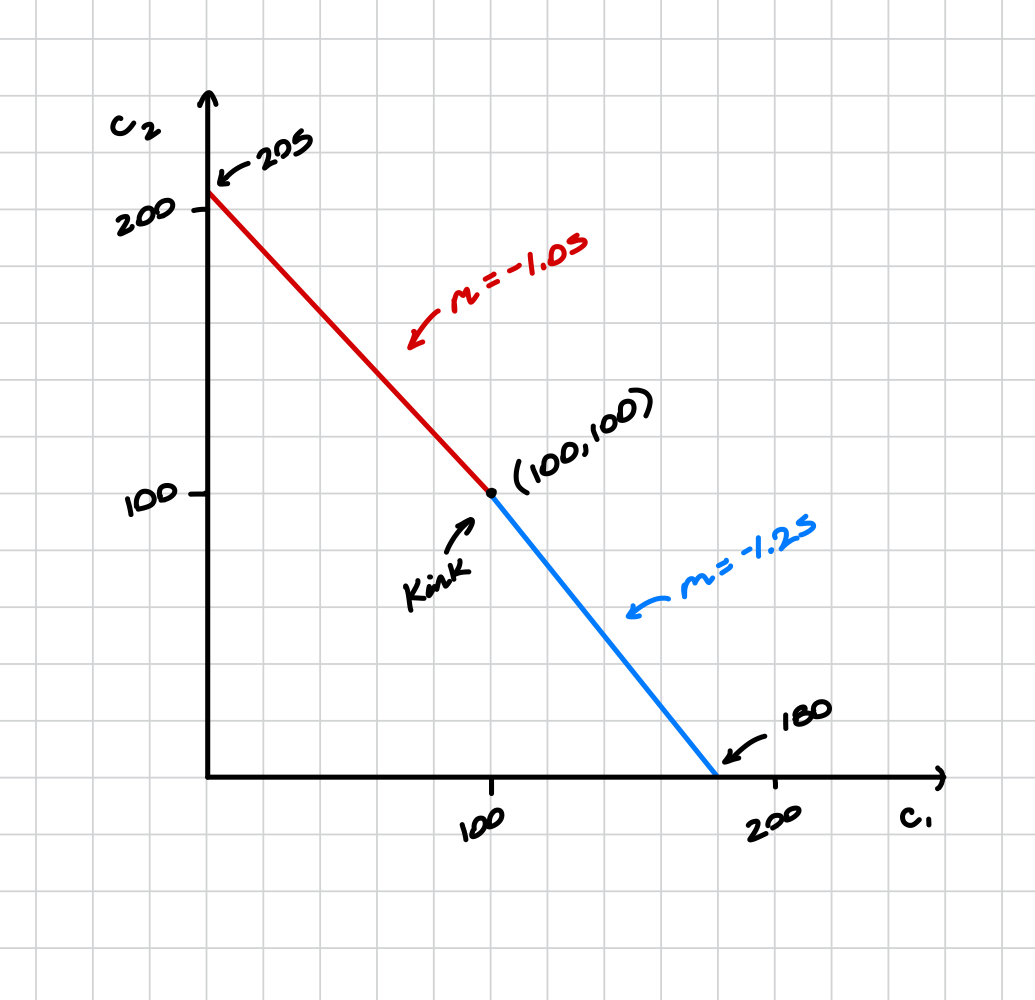
\includegraphics[width=7cm]{ECON 20000 PSet 7 Image 1.jpeg}
\item Continue to assume the interest rates in part (f) and  $m_1 = m_2 = \$100$. For which values of $\beta$ will the consumer save?
\item[] Consumer saves when $c_1<m_1$. So $c^s_1=\frac{m_1+\frac{m_2}{1+r_s}}{1+\beta}<m_1\Rightarrow\beta>\frac{1}{1+r_s}=\frac{1}{1+0.05}=0.952$.
\item  Continue to assume the interest rates in part (f) and $m_1 = m_2 = \$100$. For which values of $\beta$ will the consumer borrow?
\item[] Consumer borrows when $c_1>m_1$. So $c^b_1=\frac{m_1+\frac{m_2}{1+r_b}}{1+\beta}>m_1\Rightarrow\beta<\frac{1}{1+r_b}=\frac{1}{1+0.25}=0.8$.
\item Continue to assume the interest rates in part (f) and m1 = m2 = 100. What is the consumer’s optimal consumption bundle if $\beta=.9$? 
\item[] Since $\beta=0.9>0.8$ and $\beta=0.9<0.952$, the consumer neither borrows nor saves and the optimal consumption bundle is the kink point at $(c_1,c_2)=(100,100)$.
\end{enumerate}
\item A farmer believes that there is 50 percent chance that next season will be rainy and a 50 percent chance that next season will be normal. His expected utility is of the form: $V=.5 · ln(y_r) + .5 · ln(y_n)$, where $y_r$ denotes his income if the season is rainy and $y_n$ denotes his income if the season is normal. Suppose the farmer is choosing between 2 crops, corn and wheat, that offer the following income prospects:
\newline
\begin{tabular}{lll}
\hline \hline
& $y_n$ & $y_r$ \\
\hline
Wheat & \$28,000 & \$10,000 \\
Corn & \$19,000 & \$15,000 \\
\hline \hline
\end{tabular}
 \begin{enumerate}[label=(\alph*)]
\item  Suppose the farmer must choose to plant either corn or wheat. Which of the crops will he plant?
\item[] $V_W=0.5ln(10000)+0.5ln(28000)=9.725$. $V_C=0.5ln(15000)+0.5ln(19000)=9.734$.
\item[] Since $V_C>V_W$, the farmer will choose to plant corn.
\item Suppose the farmer can plant half his field with wheat and half with corn. Would he choose to do so (versus the scenario in part a), where must choose one or the other?
\item[] $y_n(x)=(1-x)\cdot\text{corn}_n+x\cdot\text{wheat}_n=(1-x)\cdot19000+x\cdot28000=19000+9000x$.
\item[] $y_r(x)=(1-x)\cdot\text{corn}_r+x\cdot\text{wheat}_r=(1-x)\cdot15000+x\cdot10000=15000-5000x$.
\item[] $V_M=0.5ln(y_r(0.5))+0.5ln(y_n(0.5))=0.5ln(12500)+0.5ln(23500)=9.74912$.
\item[] Since $V_M>V_W$ and $V_M>V_C$, the farmer would choose to mix his plants.
\item What mix of wheat and corn would maximize the farmer’s expected utility?
\item[] $V'(x)=\frac{1}{2}\cdot\frac{y'_r(x)}{y_r(x)}+\frac{1}{2}\cdot\frac{y'_n(x)}{y_n(x)}$. $y'_r(x)=-5000,\; y'_n(x)=9000$. $\Rightarrow\frac{1}{2}(\frac{-5000}{15000-5000x}+\frac{9000}{19000+9000x})$.
\item[] Set FOC = 0, $\frac{9000}{19000+9000x}=\frac{5000}{15000-5000x}\Rightarrow9000(15000-5000x)=5000(19000+9000x)\Rightarrow135000000-45000000x=95000000+45000000x\Rightarrow40000000=90000000x\Rightarrow x=\frac{4}{9}$.
\item[] Check max: $V''(x)=\frac{1}{2}(\frac{-25000000}{(15000-5000x)^2}+\frac{-81000000}{19000+9000x)^2}$. All terms negative, so $V''(x)<0$.
\item[] Thus ideal mix of wheat and corn is $\frac{4}{9}$ wheat and $\frac{5}{9}$ corn.
\item[] $V_{M^*}=0.5ln(y_r(\frac{4}{9}))+0.5ln(y_n(\frac{5}{9}))=0.5ln(12777.78)+0.5ln(23000)=9.74936$
\item Would the availability of wheat crop insurance (available only to farmers who grow only wheat), which has a price of \$4,000 for the policy and pays benefit of \$8,000 in the case of a rainy season, cause the farmer to change what he plants (compared to part c)?
\item[] New normal: $28000-4000=24000$. New rainy: $10000-4000+8000=14000$.
\item[] $V_{W+I}=0.5ln(14000)+0.5ln(24000)=9.816$.
\item[] Because $V_{W+I}>V_M^*$, insurance does cause the farmer to change what he plants.
\end{enumerate}
\end{enumerate}
\end{document}

\\begin{enumerate}
\item  Suppose a consumer faces the possibility of an uncertain loss of income. Income in the good state is $m_g$ and income in the bad state is $m_b$. Suppose that there is insurance available for purchase at a price of $\gamma$ per dollar of coverage. Suppose that the consumer’s preferences over consumption in the good and bad states are represented by: $U(c_1, c_2) = \pi_b ln c_b + \pi_g \alpha ln c_g$.
 \begin{enumerate}[label=(\alph*)]
\item What is the consumer’s consumption in the good state if he purchases k units of insurance?
\item What is the consumer’s consumption in the bad state if he purchases k units of insurance?
\item Suppose that insurance is available at an actuarially fair rate ($\gamma=\pi_b$). Find $k$, $c_g$, and $c_b$ as functions of $\alpha$.
\item For what value of $\alpha$ does the consumer buy complete insurance coverage?
\end{enumerate}
\item A student receives utility $U(c,e)=\sqrt c + e$ from hours of studying economics, e, and consumption, c. They spend their total awake hours, $T=16$, either studying, $e$, working, $h$. Every hour they spend working, they receive an hourly wage, $w$, which becomes the income used to buy consumption at price, $p_c$. 
 \begin{enumerate}[label=(\alph*)]
\item Write down this student's descriptive problem.
\item Write down this student's problem in the canonical form.
\item Form the Lagrangian and find the demand curve for consumption and studying economics.
\item What would happen to if hourly wage increases, keeping your full income constant?
\item What would happen to your economics consumption if hourly wage increases, allowing your full income to vary?
\end{enumerate}